\section{Introduction}
In Asch's famous conformity experiments \cite{asch1956studies, asch1955opinions, bond1996culture}, groups of participants were asked to match a line with a set of three different sized lines, one of which was of the correct size.
In reality, only one of the participants was ``real" and the others were actors who unanimously chose an incorrect choice.
On average, 25\% of participants conformed to the incorrect consensus compared to 1\% of incorrect answers in a control group.
Bias in rating systems which arise from feedback from the actions of other participants are known as \emph{Social Influence Bias} \cite{demarzo2003persuasion, moscovici1972social, wood2000attitude}.
Similar to the Asch experiment, we explore the tendency for participants to conform in recommender systems, where feedback from the community encourages future participants to enter ratings closer to what they perceive as the ``norm" \cite{banerjee1992simple}.

\begin{figure}[t]
  \centering
    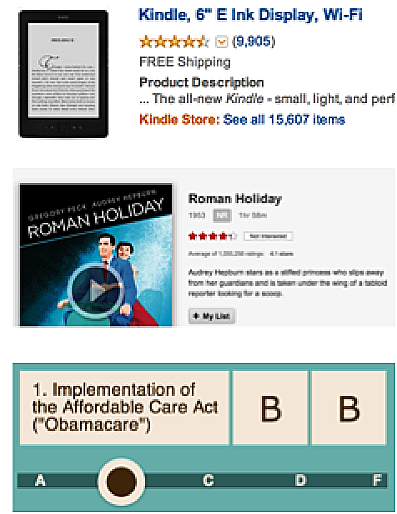
\includegraphics[scale=0.27]{../plots/intro.png}
      \caption{Multi-valued recommender systems (eg. Amazon and Netflix) are commonly used and often display aggregate statistics. The CRC is unique as it reveals the median value only after participants leave a rating and allows a participant to change his or her rating.}
      \label{grading-0}
\end{figure}

Participants in almost all recommender systems encounter results derived from the ratings of others.
For example, online retailers show the average rating for a product before a participant shares his or her rating (Figure \ref{grading-0}), and Netflix displays a personalized ``guess" for a participant's rating for an unseen movie.
Displaying the mean or median rating is desirable for browsing/selection.
Additionally, the use of social content is an established user experience design technique to incentivize participation\cite{jian2012incentive, shneiderman1992designing}, where participants are encouraged to enter more information to so they can learn more about their peers.
Furthermore, an application of particular interest is online participatory democracy where displaying results increases the transparency of the system \cite{albors2008new,o2012transparency,noveck2008wiki}.

We study social influence bias using a new platform, the California Report Card (CRC).
The CRC is a two phase recommender system: in the first phase participants enter ratings (on a 13-point scale) for six political issues, and in the second participants join a textual discussion where they read and rate the comments of others.
Phase two is a typical recommender system that uses participant ratings to build a reputation model that quickly identifies insightful comments.
Phase one is also a recommender system as it uses the six ratings to quantify similarity between participants.
The CRC has a unique rating interface that reveals median values to participants only \emph{after} they leave a rating, and then allows participants to revise ratings.
We study social influence bias in this platform, especially since tendency to conform will affect our measure of similarity between participants in phase one.
For comparison with the CRC, we ran a reference survey through SurveyMonkey with same political questions, but without displaying the median value, and it was given to a random sample of 611 participants from the company's paid pool of California participants.
To minimize assumptions about the statistical distribution of ratings, we develop a non-parametric approach to test the following social influence hypotheses:

\noindent \textbf{- Hypothesis 0} Given the opportunity, participants will revise their ratings.

\noindent \textbf{- Hypothesis 1} When a participant does change a rating it will be in the direction that conforms to the presented median.

\noindent \textbf{- Hypothesis 2} Participants will become more moderate in their ratings if they observe that their ratings consistently are in disagreement with the population consensus.

Nearly 35\% of participants changed at least one rating, and our study finds statistically significant effects of social influence bias in the $862$ out of $9390$ ratings which were changed after participant's saw the median value.
To further model patterns of participant behavior, we train a polynomial regression with the Bayesian Information Criterion (BIC) that predicts rating changes given a participant's current rating.
The model can also be inverted to infer initial ratings from final ones.
Prior results in social influence bias have focused on binary rating systems eg. up or down votes \cite{muchnik2013social, zhu2012switch}.
However, these models are not directly applicable in many recommender systems which often have discrete mutli-valued rating scales (eg. 5 stars).

Our results, which especially focus on mutli-valued ratings, have the following implications for interface and algorithmic design in recommender systems.
Few existing tools collect both an initial (with the mean/median hidden) and a final rating.
As seen in the CRC, given the opportunity to revise ratings, many participants will, and it can be informative to collect the pairs of ratings.
The pairs can reveal more information about participants' initial perceptions, allow us to classify participants as likely to conform/deviate, and also assess the magnitude of social influence from the community.
Almost all recommendation algorithms rely on an accurate characterization of participant similarity and our results suggest that social influence bias can significantly affect similarity metrics.
Existing recommender systems, can use our models to mitigate these effects, by training on set of rating pairs collected after-the-fact, and then applying the model to infer past participant's ``unbiased" ratings.

